Wolfenstein 3D was released on May, 5th 1992 and established the First Person Shooter genre. The game design supported by an engine allowing beautiful 256 colors graphics, speed, high framerate, clever I.A, crisp sounds effects and engaging musics was universally acclaimed. Within a year more than 100,000 units had been sold over the mail\footnote{The game was distributed via shareware.}, bringing fame and a little bit of fortune to the team who built it: id Software.\\
\par
\begin{figure}[H]
\centering
\fullimage{action_packed.png}
\end{figure}
\par
But the many fans did not stop at beating the game. Because they wanted to modify it and make their own characters and maps, they started to explore and reverse engineer the engine. Within a few months the assets formats were well known and people released mods\footnote{MODified version.} with altered graphics, sounds effects, music and maps. The core of the game however, the 3D engine and the secrets of its speed remained mostly unknown.\\
\\
It was kept secret for an obvious reason. A powerful engine is an essential asset for a gaming company. As a mean to outperform competitors it is a good business practice to keep other programmers clueless. Which allows to maintain a technological advantage, make betters games and generate more profit.\\
\\
But a few people within id Software did not see things that way. Instead of going along with what was common sense, they wanted to embrace players enthusiasm and fully open the source code to the public. After many internal debate, id Software did the unthinkable. On July 21, 1995 they uploaded a zip archive on \emph{ftp.idsoftware.com} containing the full source code of the engine with instructions to build it\footnote{They were not totally crazy, they had built a game engine making Wolfenstein 3D obsolete: Doom was released on December 10, 1993}.\\

 \begin{fancyquotes}
   Programming is not a zero-sum game. Teaching something to a fellow programmer doesn't take it away from you. I'm happy to share what I can, because I'm in it for the love of programming.\\
   \\
\textbf{John Carmack - Programmer}
 \end{fancyquotes}\\
\\
Opening the code did not only allow modding and educate programmers. It had two unforeseen consequences:\\
\\
First, it allowed the software to live long after the target hardware and operating system died. With access to the source, programmers were able to maintain and port the engine to new hardware and operating systems. Twenty years after the release of Wolfenstein 3D you can still play the game on anything with a CPU, some RAM and a framebuffer. \\
\\
Second, it created a window back in time looking right into 1991. Having reviewed complex engines such as Quake III and Doom III on \emph{fabiensanglard.net} I thought I would have merely skimmed over Wolfenstein 3D engine and its "simple" raycasting technology. But when out of curiosity I took a deeper look, something stroke me and I could not stop. The more I read, the more I came to realize how the target machine, the IBM PC, was designed for office work. Not for gaming. It was meant to crunch integers and display static images for word processor and spreadsheet applications. This the story this book is trying to tell. What id Software\footnote{A few other companies, such as Origins and LucasArts where also doing amazing things. I focus on Id because we have the source code!} did in 1991 was not just program a machine. What they did was re-purpose something built to do office work and turn it into the best gaming platform in the world.\\
\\
But why go through so much trouble? After all if you were a game company and you wanted to make video games, you had hardware dedicated to this very specific task: video game console! The Genesis, the Super NES and the Neo-Geo had sprite engine which albeit small limitations such as size and number allowed to move something on the screen by simply updating its $(x,y)$ coordinates. They were able to easily generate smooth animation at 60 frames per second. They had controllers, they had an audio system for sound and music. They were homogeneous (all SNES were the same configuration). If really you wanted to use a personal computer for a game why not use an Amiga 500 which was packed with coprocessors designed for animation?\\
\\
The reason fits within one word. Framebuffer. The kind of game id Software wanted to create could not be done with a sprite engine or tricks from a Copper\footnote{Nickname of a powerful Amiga co-processor allowing operations at vsync level}. They wanted to shake the gaming world by providing an immerse experience in three dimensions. And in order to do that they needed to draw a full screen, pixel per pixel, in a framebuffer before it was sent to the monitor. \\
\par
And to draw all these pixels, they also needed a powerful CPU. A PC outperformed any console on the market and no Amiga\footnote{Jimmy Maher advances an interesting theory in his book "The Future was here: The Commodore Amiga": People wanted to play First Person Shooter, which the Amiga architecture did not allow. This inability ultimately provoked the downfall of Commodore's best seller.} even with their co-processor could rivalize in terms of raw power as the mips\footnote{Million Instructions Per Second.} graph shows.
\par
\begin{figure}[H]
\centering
  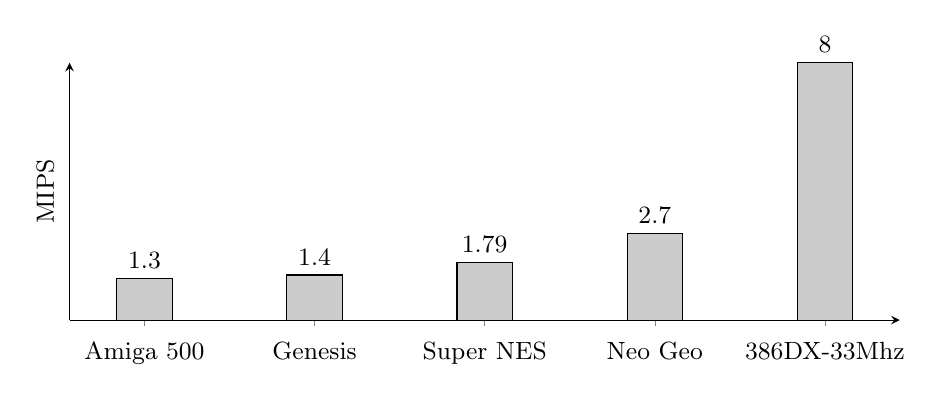
\begin{tikzpicture}[font=\small]
    \begin{axis}[
      width=\textwidth,
      height=0.4\textwidth,
      ybar=6pt,
      bar width=20pt,
      ylabel={MIPS},
      ymin=0,
      ytick=\empty,
      xtick=data,
      axis x line=bottom,
      axis y line=left,
      enlarge x limits=0.11,
      symbolic x coords={Amiga 500, Genesis, Super NES, Neo Geo,386DX-33Mhz},
      xticklabel style={anchor=base,yshift=-\baselineskip},
      nodes near coords={\pgfmathprintnumber\pgfplotspointmeta}
    ]
      \addplot[fill=black!20,draw=black] coordinates {
        (Amiga 500,1.3)
        (Genesis,1.4)
        (Neo Geo,2.7)
        (Super NES,1.79)
        (386DX-33Mhz,8)
      };
    \end{axis}
   \end{tikzpicture}
   \caption{Consoles Vs PC, CPU comparison with MIPS\protect\footnotemark \protect\footnotemark.}
   \label{fig:ems_xms_layout}
 \end{figure}
 % Latex footnote I HATE YOU !!!!!!
 \addtocounter{footnote}{-1}
 \footnotetext{Million Instructions Per Second.}
 \stepcounter{footnote}
 \footnotetext{The Amiga 500, Genesis, and Neo-Geo have a Motorola 68000 CPU respectively running at 7.16 MHz, 7.6 MHz, and 12 Mhz. The Super NES uses a WDC 65816 CPU which is a 8/16 bit version of a 6502 running at 3.58 MHz.}


 
With its fast CPU and 256K framebuffer, a 1991 PC looked promising at first. Except according to the user manual there were three seemingly impossible\footnote{The title of this book could have easily be "The Impossible Machine".} obstacles to overcome:\\
\begin{itemize}
\item The video system (called VGA) could not do double buffer: It was not possible to have smooth animations without tearing on screen.
\item The CPU could only do integer operations...yet the mathematics required for 3D involves keeping track of fractions.
\item The PC Speaker, the default sound device could only produce square waves. A bunch of "beeps" which were more annoying than anything.
\end{itemize}
On top of these major blockers lay a myriad of major difficulties:\\
\begin{itemize}
\item The RAM addressing mode was not flat but segmented resulting in complex and error prone pointer mathematics.
\item The pixel of the VGA were not square: the framebuffer was stretched vertically when
transfered to the screen.
\item The audio ecosystem was fragmented: Various sound systems had different capabilities and expectations.
\item The machine could only address 1MB of RAM. To go past that you had to enter a fragmented eco-system of drivers.
\end{itemize}

Overall, it looked like the machine was \emph{doom}ed to do boring things. But teams of people around the world did not accept that and tinkered with the hardware to achieve unexpected results. How they did it is the raison d'etre of this book. By first showing the hardware limitations I hope programmers will develop an appreciation for the software and how it navigates obstacles:
\begin{itemize}
\item Chapter I: The Hardware. The five parts of a PC from 1991.
\item Chapter II: The Team\footnote{This is an engineering book: The description is logistic. For the human aspect read David Kushner's chef d'oeuvre: "Masters of Doom''}. The people pushing the edges.
\item Chapter III: The Software. Wolfenstein 3D game engine.
\end{itemize}
\par
\bu{Trivia :} The game was inspired by the 1981 Apple II title "Castle Wolfesntein" by Silas Warner. The Apple version was stealth oriented (Wolfesntein "Profound Carnage" style was a clear departure from the original theme) but really stood out thanks to its unprecedented use of digitized voices. Initially the team believed that they would be unable to use the Wolfenstein name due to trademark issues, and came up with multiple possible titles, only to discover that the original developer, Muse Software, had gone out of business several years earlier and let the trademark lapse, leaving them the option to name their game Wolfenstein 3D.

\begin{figure}[H]
\centering
\fullimage{CastleWolfensteinC64.png}
\caption{Castle Wolfesntein}
\end{figure}
